\scanpage{51}
\margin{50}
\mspage{5}
\deleted{
\[
(20)\qquad\uline{\bar\omega}\simeq\{\pm1\}\quad\text{\inserted{if needed} i.e. we have }\uline{\omega}\xrightarrow{\sim}\uline{\varepsilon}
\]
so henceforth we identify the set $\uline{\omega}=\Omega(J)$ \inserted{$=\Omega(\Sigma_{\mathbb R})$} with the set $\uline{\varepsilon}$ of the two hemispheres.
}
\margin{These are \uline{arcs} of \unsure{one of the} circles, which are determined by origin, endpoint, designation of the circle, and direction of traversal.}
\margin{\uline{NB}
\[
\operatorname{Rep}(J)\simeq J\times\uline{\omega}
\]
\[
(i,j,k)\longmapsto(i,\omega_{i\to j\to k})
\]
the packet $(a_i^{\omega\varepsilon})$ is a torsor under $\Gamma=G_J\times\{1,\tau\}$\qquad(22).
}
Let us introduce on $\widetilde\Sigma$ the \deleted{\unsure{arcs}} simple paths : (embedded oriented segments)
\[
(21)\qquad\overbrace{a_i^{\omega,\varepsilon}}^{12},\quad
\overbrace{b_i^\omega}^{6},\quad\overbrace{c_i^\varepsilon}^{6},\quad\overbrace{d_i^\varepsilon}^{6},\qquad
i\in J,\ \omega\in\uline{\omega},\ \varepsilon\in\uline{\varepsilon}
\]
each packet \inserted{$b,c,d$} forming a torsor under $G_J$

$\tau$ acting by
\[
(22)\quad \tau a_i^{\omega,\varepsilon}=a_i^{\omega,\varepsilon'},\quad
\tau b_i^\omega=b_i^\omega,\quad \tau c_i^\varepsilon=c_i^{\varepsilon'},\quad \tau d_i^\varepsilon=d_i^{\varepsilon'}.
\]
\margin{\uline{NB} we thus have \deleted{deduced}
$g(a_i^\omega)=a_{g(i)}^{g(\omega)}$ and so on.}
We have
\[
(23)\qquad a_i^{\omega\varepsilon}:S_i^\varepsilon\longrightarrow\deleted{S_i^\varepsilon}R_i^\omega\text{ on }U_i\quad\inserted{(\text{quarter turn})}
\]
\deleted{in the direction of the orientation of $\Sigma$ at $R_i$}
which characterizes $a_i^{\omega\varepsilon}$. \deleted{makes explicit the fact that}
\[
(24)\qquad b_i^\omega:Q_i\longrightarrow R_{\omega'i}^{\omega'}\text{ on }\widetilde\Sigma_{\mathbb R}\simeq\deleted{\unsure{\Sigma_{\mathbb R}}}\inserted{\operatorname{Dec}(\Sigma_{\mathbb R},J)}\ \deleted{\text{on the}}
\]
\deleted{(path with origin on this circle)}
(path on $\widetilde\Sigma_{\mathbb R}$, with origin $Q_i$, in the direction $\omega$, up to the endpoint \deleted{\unsure{which is}} of the component segment of $\widetilde\Sigma_{\mathbb R}\simeq\operatorname{Dic}(\Sigma_{\mathbb R},J)$, namely $R_{\omega'i}^{\omega'}$.
\[
(25)\qquad c_i^\omega:P^\omega\mathrel{-\!\!\!-\!\!\!-}Q_i\qquad\text{along an arc of a great circle}
\]
\[
(26)\qquad d_i^\omega:P^\omega\longrightarrow S_i^\omega\qquad\text{along an arc of a great circle}
\]
\margin{We also set
\[
(27)\quad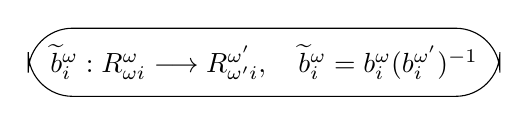
\begin{tikzpicture}[baseline=(f.base)]
\node[draw,rounded corners=16pt,inner xsep=8pt,inner ysep=6pt] (f) {$\widetilde b_i^\omega:R_{\omega i}^{\omega}\longrightarrow R_{\omega'i}^{\omega'},\quad\widetilde b_i^\omega=b_i^\omega(b_i^{\omega'})^{-1}$};
\end{tikzpicture}
\]
paths in the direction $\omega$ and not for $b_i$\deleted{\unsure{of the points}}\deleted{\illegible{3}}
}
All the arcs $\widetilde b_i^\omega,c_i^\omega,d_i^\omega$ are traced on great circles of $\Sigma$, except that the endpoints, of the $c_i^\omega,d_i^\omega$ are not in $\Sigma^*$ but in \inserted{$U_i\subset$} $\partial\widetilde\Sigma\setminus\Sigma^*$
